\label{chap:testing}

Firstly, this chapter deals with the simulation of the LSP process in RoboDK. Secondly, it focuses on testing the robotic arm program on the physical robot. The goal of the testing is to evaluate the effectiveness of the solution in the CAM program RoboDK. The robotic arm cell used for simulation and testing is depicted in section \hyperref[sec:lsp_layout]{\ref{sec:lsp_layout} LSP station layout}. A forging die is used as a test sample. Figure \ref{fig:cad} shows a CAD drawing of the forging die. Figure \ref{fig:cad} also highlights in black the areas to be treated by the LSP process and the approach/retreat motions in green. Information about the areas to be treated by the LSP process is usually provided by the manufacturers based on experience from the factory floor.

\begin{figure}[h]
    \centering
    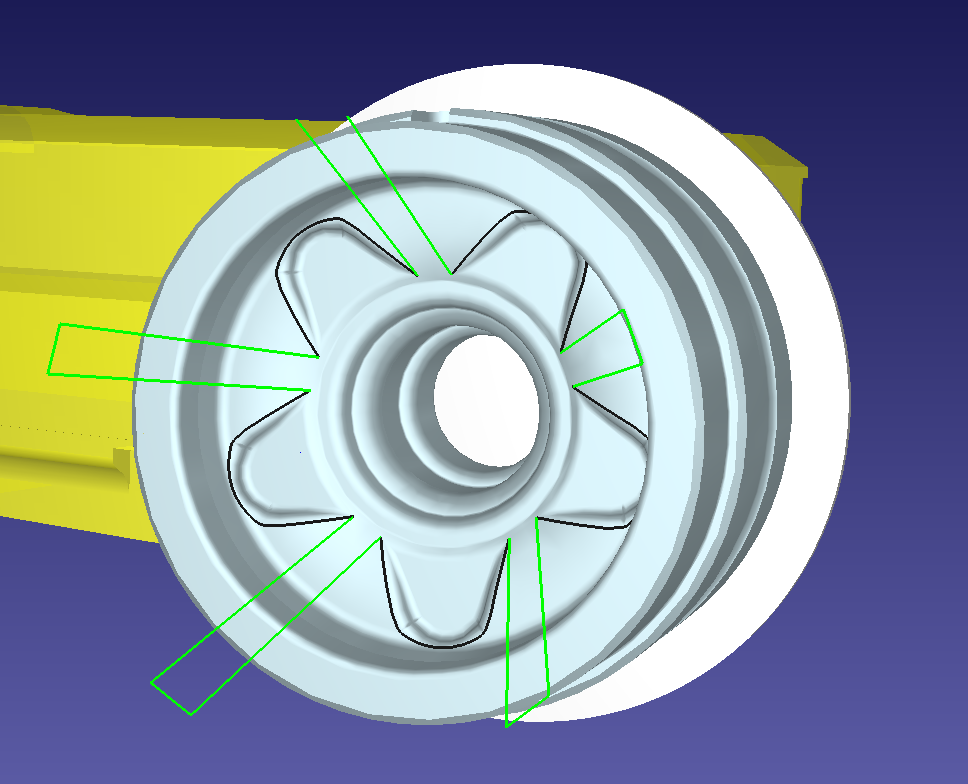
\includegraphics[width=0.8\linewidth]{img/cad.PNG}
    \caption{CAD drawing of forging die}
    \label{fig:cad}
\end{figure}

\section{Simulation}

The simulation process can be broken down into several steps:

\begin{enumerate}

\item create a robot machining project in RoboDK, so it mirrors the actual robotic arm workcell, 

\item set up the curve follow project, set appropriate collision checking parameters and successfully solve robotic arm path,

\item set appropriate simulation parameters and run simulation,
generate robotic arm program with RoboDK,

\item if simulation is sucessful, continue with testing on physical robotic arm.

\end{enumerate}

Figure \ref{fig:robodk_die} shows a picture of the RoboDK workcell with the forging die mounted onto the flange of robotic arm.

\begin{figure}[h]
    \centering
    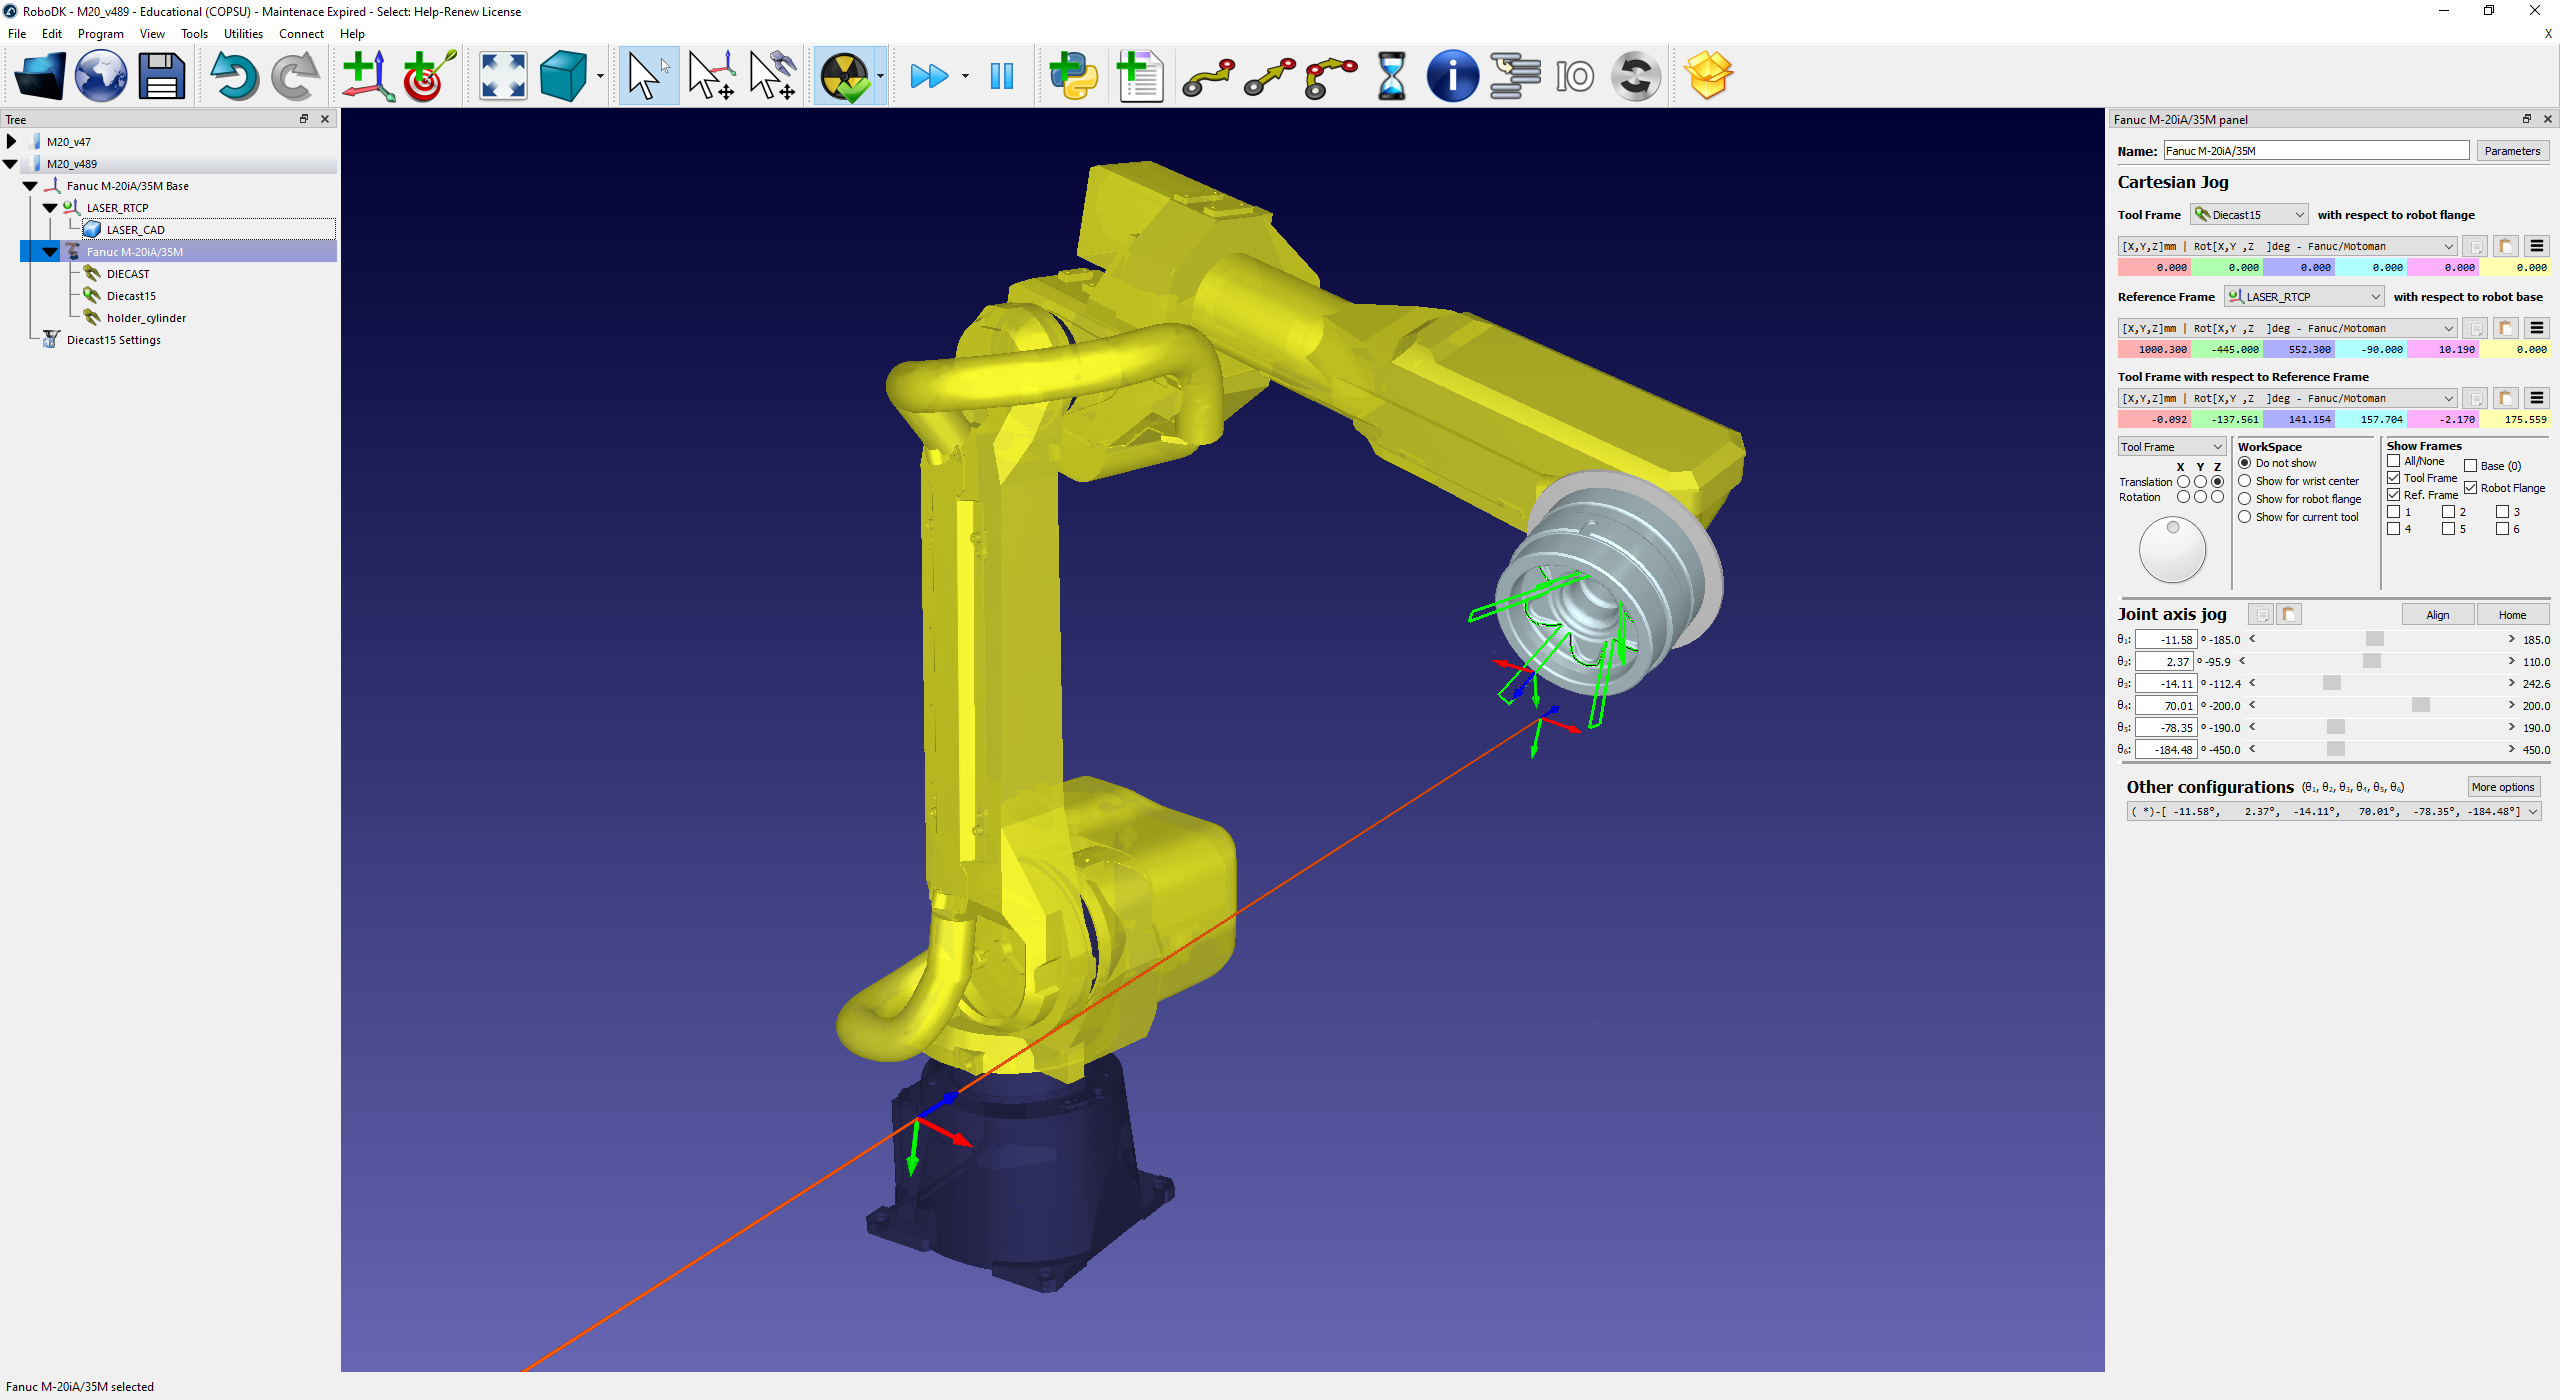
\includegraphics[width=1.0\linewidth]{img/robodk_cast.PNG}
    \caption{RoboDK workcell with forging die}
    \label{fig:robodk_die}
\end{figure}


\section{Testing on the physical robot}

The testing of robotic arm programs on physical robots follows after the simulation process and is roughly divided into the following steps:

\begin{enumerate}
    
\item upload program to robotic arm controller,

\item run program on physical robotic arm in test mode (test mode = mode of robotic arm with reduced maximum speed) and without laser source,

\item run program on physical robotic arm in production mode (production mode = speed of robotic arm is not restricted),

\item run program in production mode with active laser source. The energy of the laser source is set to a value that is appropriate for the given LSP application. 

\end{enumerate}

Figure \ref{fig:cast} shows the forging die mounted on the robotic arm.

\begin{figure}[h]
    \centering
    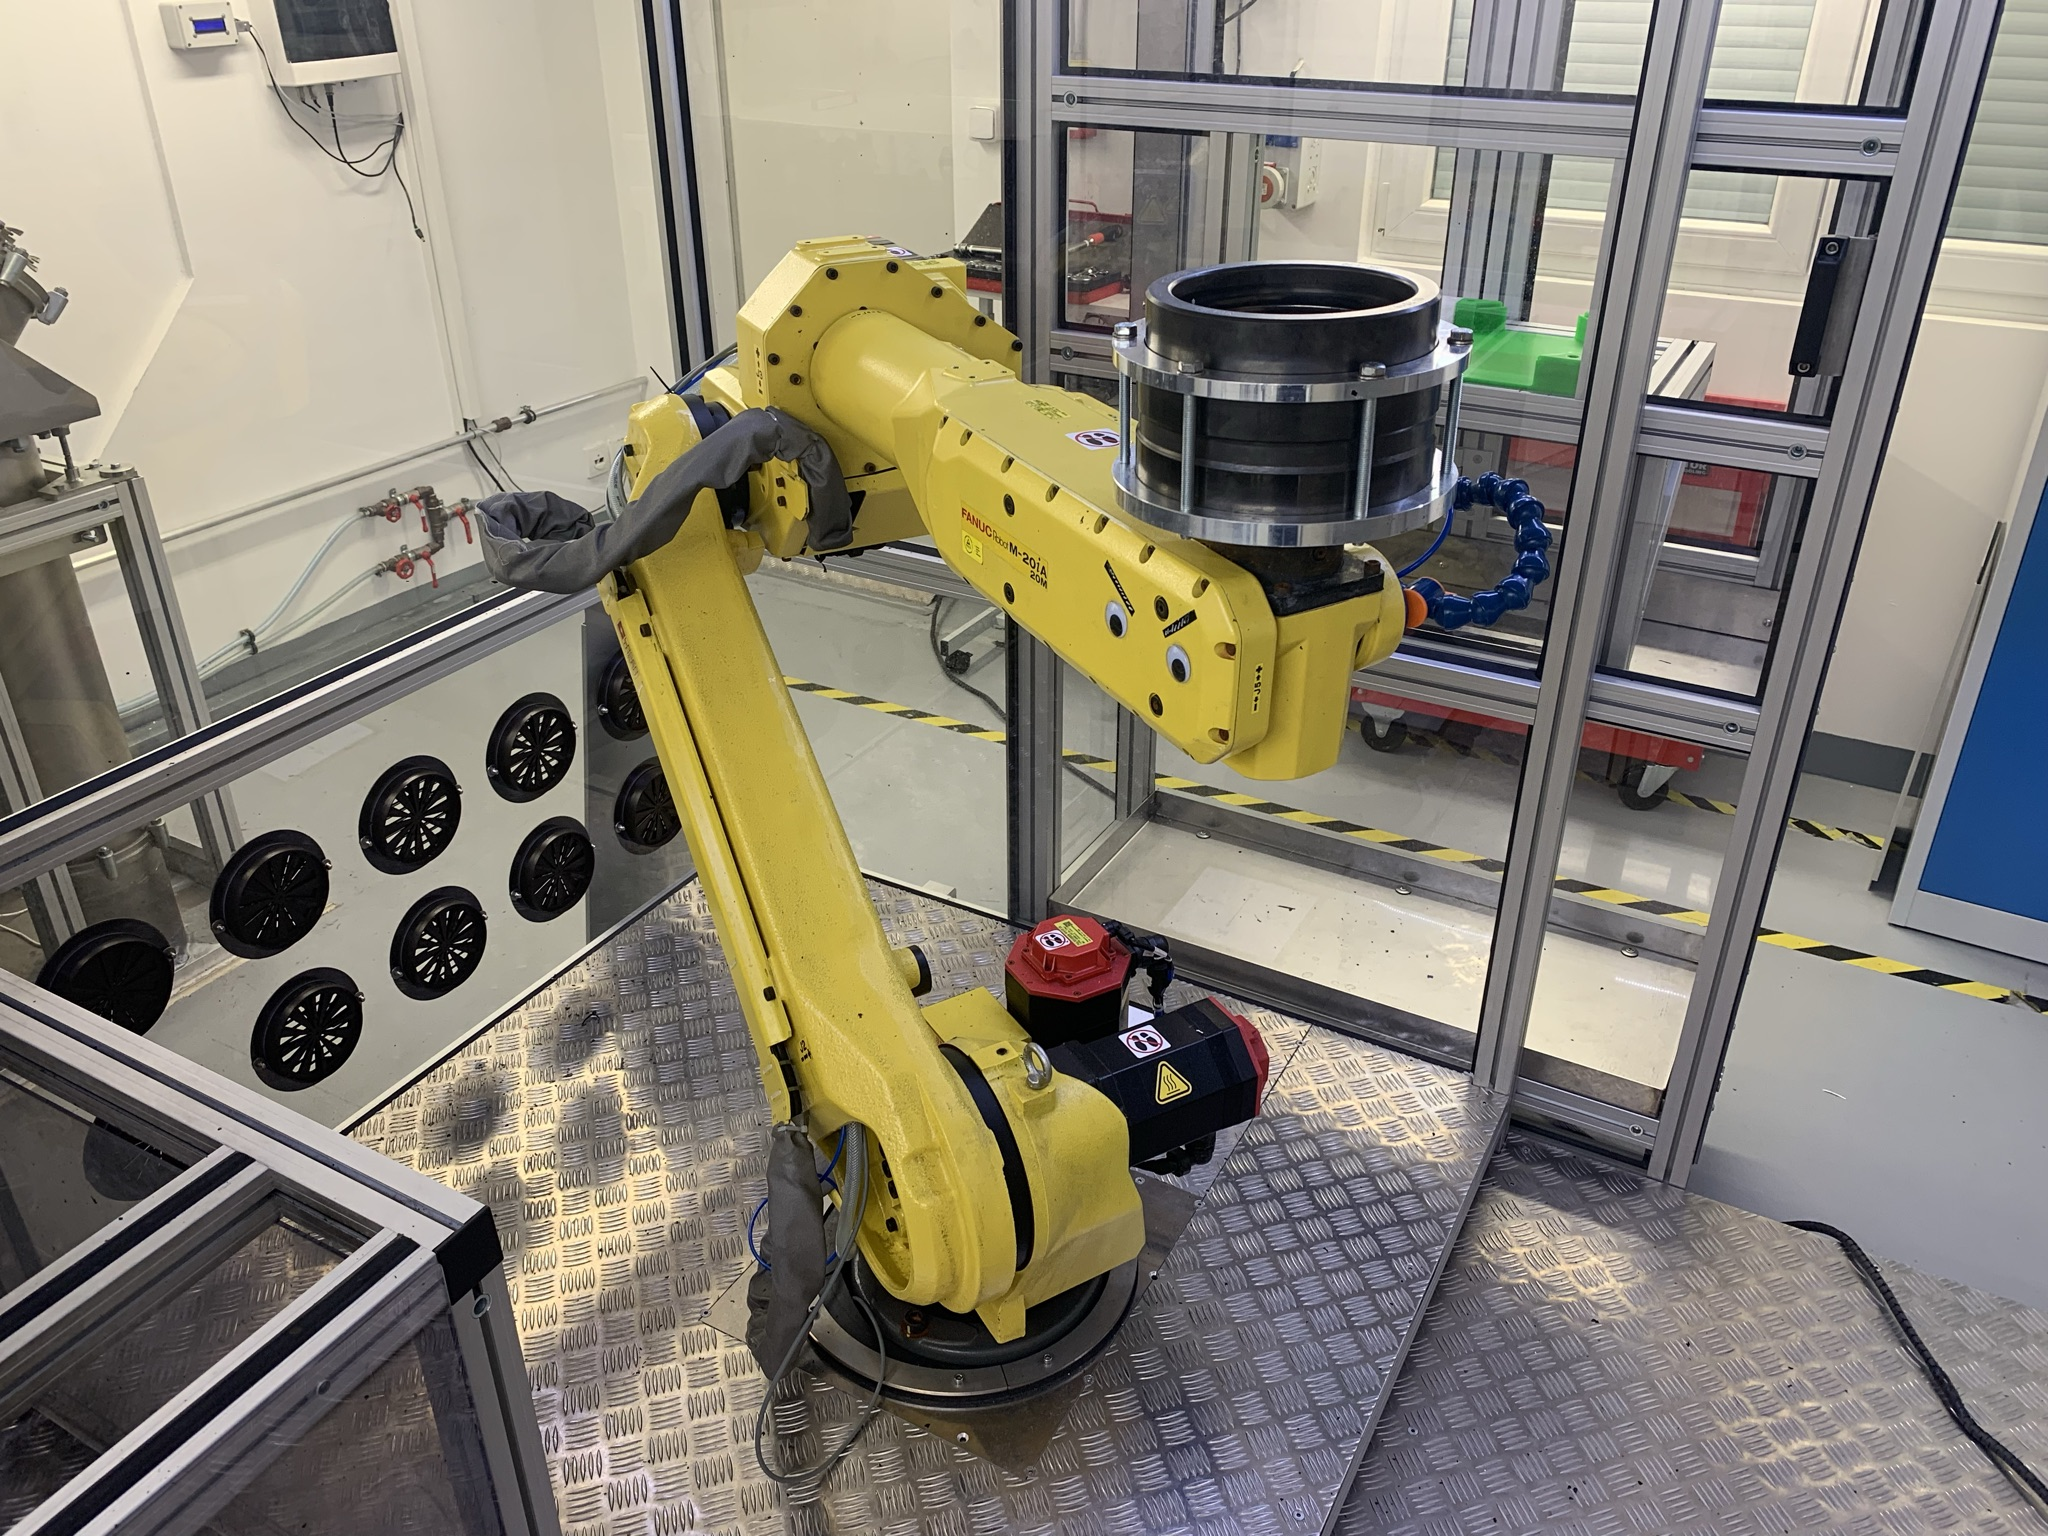
\includegraphics[width=1.0\linewidth]{img/cast.jpeg}
    \caption{Forging die mounted on the robotic arm}
    \label{fig:cast}
\end{figure}

\section{Result of testing and simulation}

Both simulation and testing on a physical robot were sucessful. Figure shows the actual LSP process performed on the forging die. 



